% ===========================================
% Introduction
% Written by: Braidan Duffy
%
% Date: 05/02/2023
% Last Revision: 05/02/2023
% ============================================

\setchapterstyle{kao}
\chapter{Introduction}
\setchapterpreamble[u]{\margintoc}
\labch{introduction}

The Self-propelled Electric Autonomous CATamaran (SEACAT) is envisioned to compete in the Promoting Electric Propulsion (PEP) competition sponsored by the American Society of Naval Engineers (ASNE).
This is an annual competition that challenges teams from the academic, public, and private sectors to design, build, and race small electric boats in a 5-mile course.
These boats can either be crewed or uncrewed and are tasked with completing the 5 single-mile laps as quickly as possible.

For SEACAT 2023, the requirements for the system are deceptively simple: 1) The vessel must be uncrewed, and 2) the vessel should be able to navigate the course autonomously via GPS waypoints.
These high level requirements drive a variety of lower-level requirements which will be discussed in Section \ref{ssec:requirements}.
For any robotic system, the control systems engineers must balance the requirements of the system with the capabilities and constraints present.
In SEACAT 2023's case, as with many other systems, the largest constraints present are time and cost, and given the limited experience available on the controls team, capabilities also had to be limited.

Therefore, we decided to leverage large, open-source communities for the backbone of our architecture.
High-level control is provided by the BlueRobotics BlueOS package which implements the ArduPilot control firmware for calculate vehicle position, attitude, course, speed, etc.
ArduPilot also integrates with Ground Control Software (GCS) like QGroundControl which allows us to easily plan missions and remotely operate the vessel.
BlueOS also provides a useful web interface for monitoring, management, and diagnostics and is in active development with integration onto USVs in mind.
For lower-level control, SEACAT utilizes the Robot Operating System version 2 (ROS2) which provides a robust publish/subscribe architecture for sensors, payloads, and control electronics.
We can leverage this architecture to maintain a distributed control schema for the vessel that maintains reliability while have multiple independent failsafe features.

To communicate between the ground station and vessel, we will be using sub-gigahertz transceivers.
These provide low-bandwidth long range communications that will allow the operators to send and receive basic telemetry from the entire length of the competition raceway.
Additionally, an independent lower-power transceiver will be used to provide a remote kill option from a chase craft following SEACAT during the competition.
Intra-system communication on SEACAT will be handled by the robust CANbus conforming to the NMEA2000 standard.
This allows SEACAT to easily incorporate different payloads and sensors in the future, while providing a resilient and standardized communication protocol

In this paper, the background, controls architecture, implementation, and testing strategies for SEACAT 2023 will be discussed.
This is intended as both a guide into our implementation of a USV control system, as well as the documentation required as a part of the PEP competition.
In the future, it is expected that this document will be updated to include relevant new information added by future teams.
These editions should be mentioned in the Revision History Table (Table \ref{tab:revision_history}) in the Appendix.

\section{Background} \labsec{background}
This section contains some of the research notes that were compiled during the design of SEACAT 2023's controls system.

\subsection{Dynamic Modelling}
One of the first steps in analyzing the control systems for a catamaran is to understand the dynamic relationship it has with the environment and itself.
To accomplish this, we need to perform a couple of steps:

\begin{itemize}
    \item Determine the physical parameters such as its dimensions, mass, and center of gravity. 
    \item Choose a reference frame that will be used to describe the position and orientation of the catamaran. 
    A common choice is an earth-fixed frame, where the x-axis points East, the y-axis points North, and the z-axis points towards space (NEU).
    \item Develop a mathematical model relating the physical parameters and the coordinate frame. 
    This typically involves writing equations of motion that describe the translations and rotational motion of the catamaran. 
    The equations of motion can be derived using techniques such as Lagrangian mechanics or Newton-Euler dynamics.
    \item Model the hydrodynamic forces acting on the catamaran, such as lift, drag, and wave-making resistance. 
    This can be done using empirical models, computational fluid dynamics simulations, or experimental data. 
    Most of this information can be found in reference textbooks.
    \item Incorporate control inputs (e.g. rudder, thruster commands), into the model. 
    These inputs can be modeled as time-varying inputs to the equations of motion.
\end{itemize}

The resulting dynamic model can be used to simulate the motion of the catamaran under various conditions and control inputs. 
This is a part of the "digital twin" and can be used to predict future states of the craft which can be useful for analyzing its stability, performance, and response to external disturbances. \sidenote{The complexity of the dynamic model will depend on the accuracy required and the intended use of the model. Simplified models may be sufficient for some applications, while more complex models may be necessary for others.}

The dynamic model will take the form of a linear, time-invariant (LTI) model expressed in the standard state-equation form.
To derive this model and program it, we must create a representation, discretize it, and then implement and plot its response.
The implementation of this model can be forwarded to more advanced artificial intelligence algorithms like Bayesian Networks or Extended Kalman Filters for filtering and smoothing.

\paragraph*{Model representation:} The LTI model is represented using the standard state-equation form, which expresses the state of the system in terms of the state variables and their derivatives. The state equation is usually expressed as a set of first-order linear differential equations:

\begin{gather} \labeq{lti_start}
    \frac{d\vec{x}}{dt} = A\vec{x} + B\vec{u} \\
    \vec{y} = C\vec{x} + D\vec{u} \\
    \begin{aligned}
        \text{where } & \vec{x} \text{ is the state vector,} \\
                      & t \text{ is time,} \\
                      & A \text{ is the state-transition matrix,} \\
                      & B \text{ is the input-to-state matrix,} \\
                      & \vec{u} \text{ is the control input vector,} \\
                      & \vec{y} \text{ is the state output vector,} \\
                      & C \text{ is the state-to-output matrix, and } \\
                      & D \text{ is the direct-transformation matrix}.
    \end{aligned} \notag
\end{gather}

\paragraph*{Discretization:} To program the response of the LTI model, the continuous-time model needs to be discretized. 
This can be done using techniques such as the forward Euler method, the backward Euler method, or the trapezoidal method. 
The discrete-time state-space representation of the model is given by:

\begin{gather}
    \vec{x}_{n+1} = A \vec{x}_n + B \vec{u}_n \\
    \vec{y}_n = C \vec{x}_n + D \vec{u}_n
\end{gather}
    
\subsubsection{Kalman Filter} 
We can integrate these equations into a Kalman filter which fuses a process model and a measurement model to estimate the current state of the system and associated uncertainties.
The process model is represented by the state-equation form, while the measurement model is represented by the relationship between the true state of the system and the measurements obtained from sensors.
We can express the latter as:

\begin{gather}
    \vec{z}_n = H\vec{x}_n + \vec{v}_n \\
    \begin{aligned}
        \text{where } &\vec{z}_n \text{ is the current measurement vector,} \\
                      &H \text{ is the observation matrix,} \\
                      &\vec{v}_n \text{ is the current measurement noise vector}
    \end{aligned} \notag
\end{gather}

In a Kalman filter, the gain ($K_n$) is defined by the ratio of estimate and measurement uncertainties and is calculated at every filter cycle.
It broadly describes how much the filter relies on its estimate of the system states versus the measurements from the inputs.
A higher gain indicates a heavier reliance on the measurement and vice versa.
The Kalman gain is bounded by: $0 <= K_n <= 1$ and defined as:

\begin{equation} \labeq{kalman_gain}
    \begin{aligned}
        K_n &= \frac{\text{Estimate Uncertainty}}{\text{Estimate Uncertainty + Measurement Uncertainty}} \\
            &= \frac{p_{n-1}}{p_{n-1} + r_n}
    \end{aligned}
\end{equation}

We can therefore determine a \textit{State Update Equation} that uses this gain to estimate the current system state:

\begin{gather} \labeq{kalman_state_update}
    \begin{aligned}
        \vec{x}_{n} &= \vec{x}_{n-1} + K_n(\vec{z}_n - \vec{x}_{n-1}) \\
                    &= (1-K_n)\vec{x}_{n-1} + K_n \vec{z}_n
    \end{aligned} \\
    \begin{aligned}
        \text{where } &\vec{x}_n \text{ is the current state estimate,} \\
                      &\vec{x}_{n-1} \text{ is the previous state estimate,} \\
                      &K_n \text{ is the current Kalman gain and,} \\
                      &\vec{z_n} \text{ is the current measurement vector}
    \end{aligned} \notag
\end{gather}

\marginnote[-1.5in]{\textbf{Important note:} When measurement uncertainty is very large, and the estimate uncertainty is small, $K_n << 1$, hence big weight to the estimate and small weight to the measurement. When the opposite is true, $K_n -> 1$, meaning a large weight to the measurement and a small weight to the estimate. This is how the Kalman filter can regulate and smooth out noisy data by knowing the uncertainties.}

Now that we have an estimate of the current system state, we can determine the associated uncertainty with it using the \textit{Estimate Uncertainty Update Equation}. \sidenote{Also referred to as the \textit{Covariance Update Equation}.}
The estimate uncertainty should approach (converge) to 0 with each filter iteration as the filter improves its guessing accuracy.
However, if the measurement uncertainty is large (i.e. $K_n << 1$), the estimate uncertainty will converge more slowly.
The opposite is true if the measurement uncertainty is small.
In other words, the more precise your measurements are, the faster the Kalman filter will converge on the best estimate.

\begin{gather} \labeq{kalman_estimate_uncertainty}
    p_{n} = (1-K_n)p_{n-1} \\
    \begin{aligned}
        \text{where } &p_{n} \text{ is the estimate uncertainty at the current state} \\
                      &K_n \text{ is the Kalman gain at the current state} \\
                      &p_{n-1} \text{ is the estimate uncertainty of the previous state}
    \end{aligned} \notag
\end{gather}

Now that we have the current uncertainties, the Kalman filter can also predict the future uncertainties using the \textit{Estimate Uncertainty Extrapolation Equation}. \sidenote{Also referred to as the \textit{Covariance Extrapolation Equation}}
Like with the State Extrapolation Equations, this is done with dynamic models and will be unique to every example.
This future uncertainty is expressed by the variable, $p_{n+1}$

Additionally, there are uncertainties in the system's dynamic model because the real-world does not perfectly match our mathematical assumptions.
Uncertainty is caused by unanticipated changes in the system due to external factors.
This can be drift caused by ocean current, wind blowing a rocket to the side, drag, friction and, even time dilation in extreme cases.
Generally, these uncertainties can be combined into the Process Noise gain denoted by "$q$"
To account for process noise, it must be included in the Estimate Uncertainty Extrapolation Equation:

\marginnote{If the model is not known to be good or is very noisy, we can increase the process noise gain to reduce the lag error.}

\begin{equation}
    p_{n+1} = p_n + q
\end{equation}

In summary: the filter is initialized with a first guess ($\vec{x}_{0}$) and an associated uncertainty ($p_{0}$). \sidenote{These are generally null or the best guess for the starting state.}
These values are passed into the dynamic model equations and the Estimate Uncertainty Extrapolation Equation to predict the state at the first measurement ($\vec{x}_{1}$) and the associated uncertainty ($p_{1}$).
This is shown as Step 0 in Figure \ref{fig:kalman_filter}.
Then, we can take a measurement ($\vec{z}_n$) and record its uncertainty ($r_n$), using the latter to determine the Kalman gain with Equation \ref{eq:kalman_gain}.
We can then estimate the current state value using Equation \ref{eq:kalman_state_update} using the recorded measurement and the Kalman gain.
The current state estimate and its uncertainty can then be outputted from the filter and used in applications; this process is shown as Steps 1, 2a, and 2b in the figure below.
These values are then fed into the dynamic model to predict the next state and estimate the associated uncertainty (Step 3 in the below diagram).
Optionally, these predicted values can be outputted from the model as well, as the application requires.
This process typically repeats at a refresh rate of $\Delta t$ for every measurement where $n$ increments with every iteration.

\begin{figure*}[h!]
    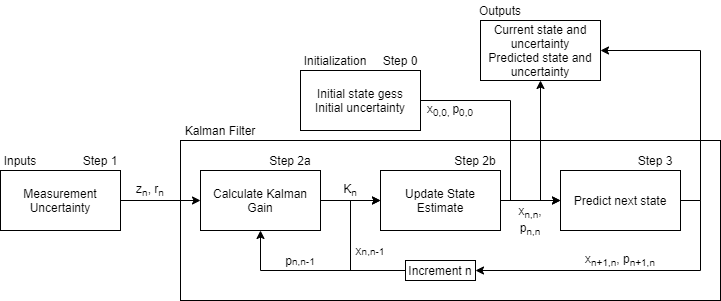
\includegraphics[height=3in]{1_introduction/KalmanFilter.png}
    \caption[Kalman Filter Diagram]{Process diagram for a Kalman filter.}
    \labfig{kalman_filter}
\end{figure*}

\paragraph{Implementation:} The discrete-time state-space representation can be implemented in a programming language, such as Python, C++, or MATLAB, to generate the response of the LTI model to a given input. 
This can be done by updating the state vector at each time step based on the state equation, and computing the output based on the output equation. The input can be specified as a time-varying function or a sequence of values.
Kalman filters are pretty-well documented and understood so multiple libraries in multiple languages exist that already implement the algorithm.

\paragraph*{Plotting the response:} The response of the LTI model can be plotted over time to visualize the behavior of the system. 
This can be useful for analyzing the stability, performance, and robustness of the system, which helps operators tune and diagnose the sensors and models.

\subsection{BlueOS/ArduPilot}
BlueOS is a new robotic platform psuedo-operating system designed for the Raspberry Pi (\todo{cite}) developed by BlueRobotics.
It runs in a Docker environment and containerizes several software packages, making it easy to deploy on a variety of systems.
BlueOS offers a web-based interface for monitoring and control of a variety of features, making it ideal as a middleware solution.

One of the most powerful packages that operates within the BlueOS container is the ArduPilot firmware (\todo{cite}).
This firmware is developed by the ArduPilot foundation and is one of the largest open-source autopilot solutions in the hobbyist market.
It has multiple variations for land, air, and water vessels and standardizes controls and autopilot commands through the Micro Air Vehicle link (MAVlink) protocol.
This allows many devices from different manufacturers to seamlessly work together.

BlueRobotics developed a Navigator HAT for the Raspberry Pi that fits atop the board and integrates seamlessly with the ArduPilot firmware.
This allows a power single board computer to read sensors, perform sensor fusion, and report the system status much faster and at a higher resolution than similar counterparts running on smaller microcontrollers.
However, the clear downside of this system is that the Raspberry Pi runs a full operating system, meaning it is susceptible to process crashes, memory overload, and other problems.
On a microcontroller, the code would instantly restart after encountering an issue.
However, on a Raspberry Pi, the code may take upwards of a minute to fully restart, if it does at all, and that means a potential loss of the vehicle.
Mitigations and contingencies for this system are described in future chapters.

\subsection{Robot Operating System 2}
ROS2 (\hl{cite: ROS2}) is a flexible and powerful open-source software framework for robot programming, and can be used to develop and implement control systems for a wide range of robotic platforms, including autonomous surface vehicles. 
In ROS2, various modules and algorithms can be implemented and connected to perform different tasks such as navigation, obstacle avoidance, and control. 
ROS2 provides a large library of packages and extensive documentation on how to write and implement your own packages. 
This enables a robust open-architecture solution where packages, services, and nodes can be customized and added to perform any functionality required by the system.
ROS2 is also lightweight enough to be deployed on edge devices such as the Raspberry Pi 4, enabling a low cost and low SWaP capability on SEACAT.

\subsection{Extra-vessel Communication}
At the farthest range, SEACAT is estimated to be close to two miles away from the ground station.
This means that powerful long distance radios must be used in order to maintain a good telemetry link with the vessel for monitoring and remote control.
In the United States, the most popular long-range frequency in use for the Internet of Things and other communities is 915 Mhz.
This band is unlicensed meaning that operators do not need to be certified to operate radios and it has a desirable resilience to obstacles while balancing an adequate data bandwidth.
SEACAT will have two radios in this band: a high gain transceiver for main communication to the ground station, and a lower bandwidth, longer range radio for an emergency craft kill switch.

The latter radio will use Long Range, or LoRa, modulation which is a wireless communication technology that enables long-range, low-power communication between devices, particularly in Internet of Things (IoT) applications. 
It is a proprietary modulation technique developed by Semtech Corporation. 
It uses spread-spectrum technology to communicate over long distances while consuming little power. 
The spread-spectrum modulation technique makes LoRa communication more resilient to interference. 
Its long-range capability allows devices to communicate over several kilometers, depending on the environment and line of sight. 
LoRa also employs a star network topology, where many end devices communicate with a single base station or gateway. 
The gateway acts as a bridge between the end devices and the network server, which can be connected to the internet. 

In robotics applications, commands can be sent from a command and control station far away from the vehicle.
The resiliency of LoRa allows for a strong connection over long distances and decreases the likelihood of communications faults due to interference.
However, the low data rate hinders operator's options for sending and receiving telemetry.
For instance, video streams are not possible with a LoRa connection as they require too much bandwidth.

\subsection{CAN Overview}
Controller Area Network (CAN) is a serial communications protocol that supports distributed real time control with high level security (\hl{cite: BOSCH CAN Specification}), and is typically used to interconnect a network of modules or nodes using a two wire, twisted pair cable.
CAN is a multimaster, multicast protocol; provided the bus is free, any node can send a message (multimaster) and all nodes can receive and act upon a message (multicast). 
The node initiating messaging is denoted as the transmitter, and any node not sending a message is called a receiver. 
CAN messages are up to 8 bytes of data and contain no explicit addresses. 
Rather, messages can be considered to be contents-addressed, where their contents determine their address. 
A message identifier is used to describe the data contents which receivers can choose to use or ignore. 
While there is no method for sending a message to a specific node, hardware can provide local filtering that allows individual nodes to react only to relevant messages.
Each message is also assigned a static priority.
When a transmitter is using the bus, it is still classified as a transmitter until the bus idles or the transmitter is supplanted by another node with a higher priority.
This methodology is called arbitration and prevents messages from being transmitted over top each other.

At a high level, CAN can be subdivided into three distinct layers:

\begin{enumerate}
    \item CAN object layer
    \item CAN transfer layer
    \item Physical layer
\end{enumerate}

The object and transfer layers are composed of the services and functions of the data link layer. The object layer functionality includes:

\begin{itemize}
    \item Finding which messages are to be transmitted 
    \item Deciding which messages received by the transfer layer are to be used
    \item Provide an interface to the application layer related hardware
\end{itemize}

In the object layer, each message transmitted over the CAN bus is represented by a CAN frame, which includes several fields, such as:

\paragraph*{The identifier field} which identifies the source and destination nodes for the message. 
The identifier field is a 11-bit or 29-bit field \sidenote{in the \textit{extended} format} in the CAN message frame that identifies the message's priority and contents. 
A receiving node can read the identifier field and determine whether to react or ignore the frame according to its purpose. 
Within the identifier field are two other fields: the message priority and the Request to Transmit (RTR).
The message priority is indirectly determined by the value of the identifier; the lower the value, the higher the message priority.
The RTR asks an appropriate receiving node to transmit data with the identifier requested.

\paragraph*{The data field} which contains the actual data being transmitted. 
The data field of a CAN message frame can contain up to 8 bytes of data. 
This data can represent anything that needs to be transmitted between devices, such as sensor data, commands, or status information. 
The data is stored in a contiguous array of bytes, with each byte representing 8 bits of information.
The actual meaning of the data in the message depends on the application that is using the CAN bus. 
For example, if a frame is used to transmit sensor data, each byte of the data field may represent a different sensor value, and the values may need to be combined or interpreted in a specific way by a receiver node to properly work.

\marginnote[-1in]{It's worth noting that not all CAN messages need to have data in the data field. 
Some CAN messages may be used only for signaling or control purposes, and may not contain any actual data. 
In this case, the data field would be empty, and the length of the data field in the CAN message frame would be 0}

\paragraph*{The control field} contains information about the type of message and any error conditions that may be present. 
The control field in a CAN message frame is a 6-bit field that contains several control bits used to manage the transmission and reception of messages on the CAN bus. 
This field includes the following bits:

\begin{itemize}
    \item \textbf{Data Length Code (DLC)}: A 4-bit field that specifies the length of the data field in bytes. The DLC value can range from 0 to 8 bytes.
    \item \textbf{Reserved Bit}: A reserved bit that is set to 0 and should be ignored by the receiving device.
    \item \textbf{Remote Transmission Request (RTR)}: As mentioned earlier, this bit is used to distinguish between data frames and remote frames. If the RTR bit is set, it indicates that the message is a request for data.
    \item \textbf{Identifier Extension Bit (IDE)}: In an extended CAN message, this bit is set to 1 to indicate that the identifier field contains a 29-bit extended identifier. In a standard CAN message, this bit is set to 0.
    \item \textbf{Error State Indicator (ESI)}: This bit is set to 1 by the transmitting device to indicate that an error occurred during the previous transmission. It is used to synchronize the error state between devices on the bus.
    \item \textbf{R0 and R1}: Reserved bits that are set to 0 and should be ignored by the receiving device.
\end{itemize}

The control field is used by both the transmitting and receiving devices to manage the transmission and reception of messages on the bus. 
The DLC and RTR bits are particularly important, as they determine the length of the message and whether it is a request for data or a message containing data. 
The IDE bit is used in extended CAN messages to indicate that the identifier field contains an extended identifier. 
The ESI bit is used to synchronize the error state between devices on the bus. 
The reserved bits should always be set to 0 and ignored by the receiving device.

The object layer can also define custom messages and message formats that are specific to a particular application. 
For example, in an autonomous surface vehicle, the object layer might define messages that are used to transmit data from the vehicle's sensors to its on-board computer, or messages that are used to control the vehicle's actuators.
The transfer layer is predominately concerned with the transfer protocol.
That is, determining bus availability, starting a new transmission, or handling an incoming message. 
It delivers messages received to the object layer and accepts messages transmitting from it. 
The transfer layer also directs bit timing and synchronization, message framing, arbitration, acknowledgement, error detection/signalling, and fault confinement.

The physical layer of the CAN bus is responsible for the physical aspects of the communication. 
It includes the electrical characteristics of the communication medium, such as the voltage levels, signaling rates, and cable impedance. 
The physical layer also includes the connectors, wiring, and termination resistors used to connect the nodes on the network. 
This also incorporates the physical addressing scheme used to identify the nodes on the network. Each node is assigned a unique identifier, which is used to identify the source and destination of the messages being transmitted.

 Each node is connected to a two-wire bus, which consists of a CAN-High (CANH) and CAN-Low (CANL) wire. 
 These wires are used to transmit differential signals that are used to represent the bits in the packet. 
 For a logical 0 or "dominant" bit, the low and high sides are driven away from each other, increasing the voltage potential between them.
 For a logical 1 or "recessive" bit, the low and high sides are driven closer together, reducing the voltage potential. When a recessive bit (logical 1) is transmitting, both CAN-High and CAN-Low are driven to 2.5 volts (indicating the voltage difference is zero during transmission of the recessive bit); when a dominant bit (logical 0) is transmitted, CAN-High goes to 3.5 volts and CAN-Low to 1.5 (voltage difference of the dominant bit is 2 volts. 
 If two nodes attempt to publish on the bus simultaneously, the dominant bit will be selected through arbitration \sidenote{The lower the value of the identifier, the higher priority to win arbitration, thus the right to publish data first on the bus.}
 An example of this can be seen in the figure below:
 
 \begin{figure}[!h]
    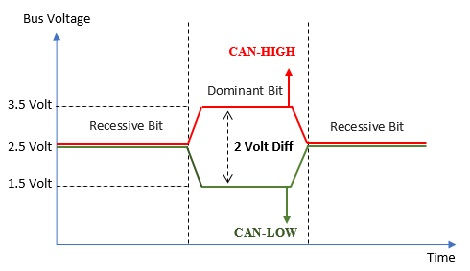
\includegraphics[]{1_introduction/CAN Differential signal.jpg}
    \caption{(\hl{Avatefipour et al., 2018}) CAN bus bit transition and signal voltages}  
    \labfig{can_signal}
\end{figure}

When a node on the CAN bus wants to transmit a message, it first checks if the bus is idle. 
If the bus is idle, the node can start transmitting its message. 
The message is transmitted as a series of frames, each of which consists of seven fields:

\begin{enumerate}
    \item \textbf{Start-of-frame (SOF)}: A single dominant bit that signals the start of a frame. 
    This bit is used to synchronize the receiving node's clock with the transmitting node's clock.
    \item \textbf{Arbitration field}: The identifier field of the frame, which includes the identifier of the message being transmitted, and is used to determine message priority during arbitration. 
    The identifier is typically a standard 11 bits (CAN 2.0A specification) or an extended 29 bits (CAN2.0B) long.
    \item \textbf{Control field}: The control field of the frame includes information about the type of message being transmitted and any error conditions.
    It contains several subfields, including the data length code (DLC) field, which specifies the number of bytes of data being transmitted and the request flag, which prompts the receiver to send a packet with the same message identifier. 
    \item \textbf{Data field}: The data field of the frame includes the actual data being transmitted, which can be up to 8 bytes long.
    \item \textbf{CRC field}: The cyclic redundancy check (CRC) field, which is used to detect errors in the message. 
    The transmitter node calculates a CRC value based on the contents of the arbitration, control, and data fields, and includes this value in the frame.
    The receiver node performs the same calculation and compares the calculated CRC value to the value received in the CRC field to check for errors.
    \item \textbf{Acknowledge (ACK) field}: The acknowledge field signals that the message has been received correctly. 
    If the message is received without errors, the receiving node sends a dominant ACK bit back to the transmitting node. 
    If an error is detected, the receiving node sends a recessive ACK bit back to the transmitting node.
    \item \textbf{End-of-frame (EOF)}: A series of seven recessive bits that signal the end of the frame.
\end{enumerate}

This frame format is summarized by the following figure:

\begin{figure}[h!]
    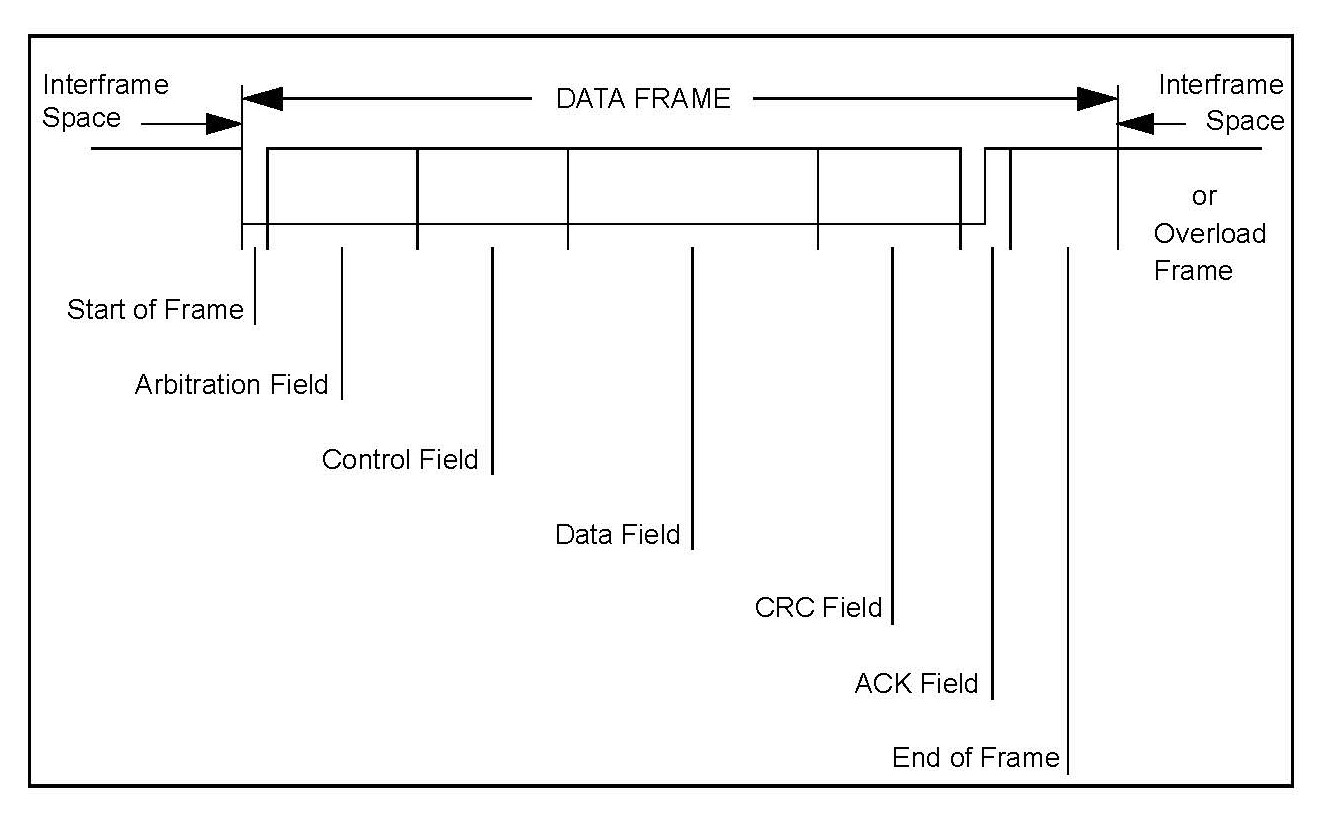
\includegraphics[]{1_introduction/CAN_frame.jpg}
    \caption[]{Breakdown of a standard CAN frame.}
    \labfig{can_frame}
\end{figure}

\subsubsection{SocketCAN}
SocketCAN is a set of open source CAN drivers and a networking stack that provides a standardized Linux socket interface for accessing CAN buses. 
It allows developers to communicate with CAN devices from user-space applications using standard socket APIs, which simplifies the development of CAN-based applications on Linux. 
SocketCAN has been included in the Linux kernel since version 2.6.25 and is widely used in industrial, automotive, and other embedded systems. 
The SocketCAN package is a Linux implementation of CAN protocols. 
It uses the Berkeley socket API and the Linux network stack; treating CAN device drivers as network interfaces. 
The framework provides a socket interface for user space applications and expounds upon the Linux network layer where CAN controller hardware device drivers are registered with the network layer as network devices, allowing CAN frames from the controller to be passed to the network layer. 

\begin{figure}[!h]
    \centering
    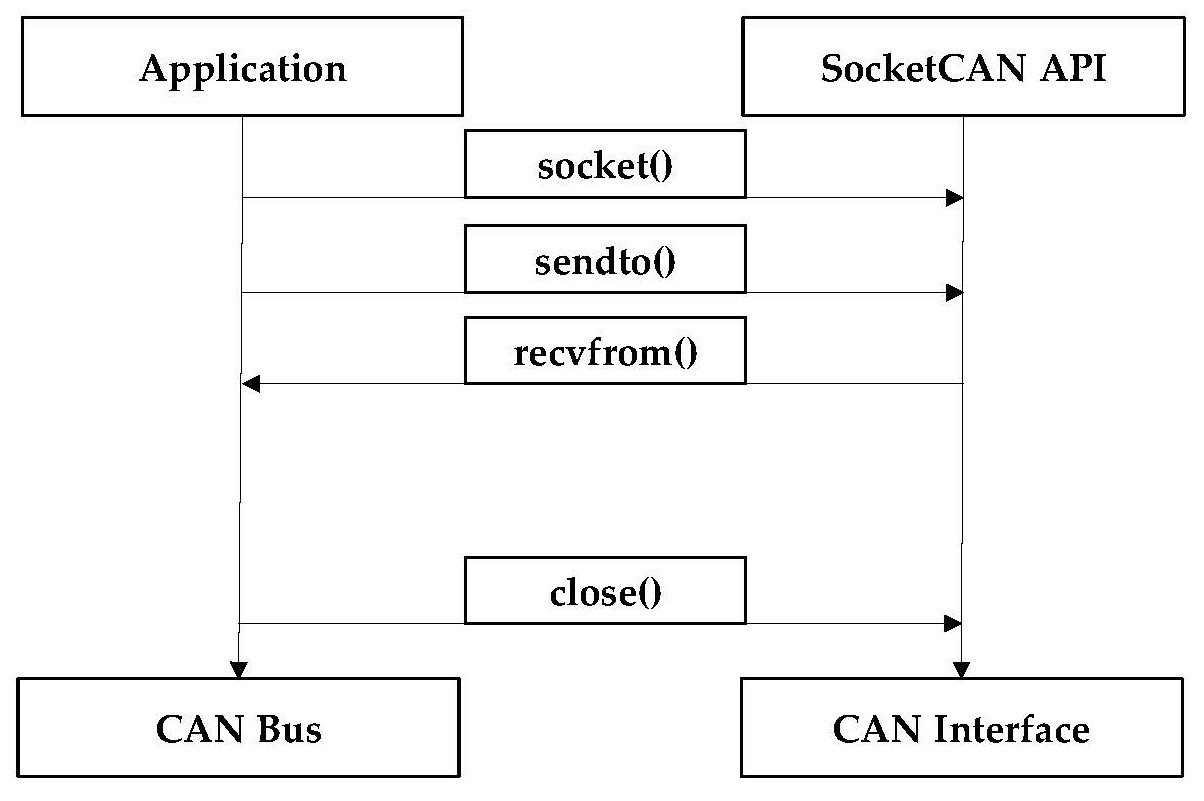
\includegraphics[]{1_introduction/SocketCAN.jpg}
    \caption{Application using SocketCAN API to communicate with CAN bus}
    \labfig{socket_can}
\end{figure}

In SocketCAN, functions can be used to configure and control the CAN interface and socket. 
The header libraries included provide definitions and declarations for the functions and data structures used in the API. 
The \lstinline{socket()} function is used to create a new SocketCAN socket that is bound to the CAN interface. 
The \lstinline{sendto()} function is used to send messages to the bus, and the \lstinline{recvfrom()} function is used to receive messages from the bus. 
After the application is finished using the socket, the \lstinline{close()} function releases the socket, freeing up associated resources. 
On the other side of the flowchart in Figure \ref{fig:socket_can}, the CAN interface communicates with the physical CAN bus.
The SocketCAN driver in the Linux kernel provides a standardized interface accessing the CAN interface and controlling the flow of messages to and from the application. 
Additional functions can be used to control the CAN interface and socket.

\subsubsection{CanKing}
Kvaser's CanKing (\hl{CITE: Kvaser}) is a Windows program for CAN bus monitoring and general-purpose diagnostics, particularly excelling as an interactive development and testing. Its features include:

\begin{itemize}
    \item Send/Receive CAN and Extended CAN messages
    \item Supports CAN FD, both ISO non-ISO
    \item Log to File (up to 4 channels)
    \item Filter Messages
    \item Generate Error Frames
    \item Timed Transmission 
    \item History Transmit List
    \item Traffic Generator 
    \item Virtual CAN Channels 
    \item Specify Custom Bus Parameters 
\end{itemize}

All of these features make it an invaluable tool for diagnostics and testing CANbus networks.

\subsection{Sensing and Models}
USVs have to be able to understand themselves and their surroundings in order to operate effectively.
There are two types of models that semi- or fully-autonomous systems must be able to construct online (in real-time): the world model, and the local model.

The world model represents all of the external factors that affect the USV's operation.
This includes other ship traffic, weather, water conditions, obstructions, landmarks, GPS coordinates, operator commands, etc.
Typically, the USV will build a world model by fusing different data streams together to formulate a best guess of its surroundings.
If, for example, we have an AIS radio that tells the USV other ships' positions and trajectories, we can fuse that information with RADAR tracks and superimpose them together.
Not all ships may be transmitting AIS, so we need RADAR to actively spot and track them; conversely, not all ships may appear properly on RADAR, but their AIS signals will allow the USV to estimate their position.
By fusing these two data streams together, the USV can have a highly confident estimation of the traffic around it and maneuver accordingly.

Similarly, the USV has to understand its internal data to understand its own capabilities and limitations.
Sensors like strain gauges, voltage monitors, ammeters, accelerometers, fuel gauges, etc. all feed data to the USV's central computer to inform it of its own health.
In our particular case, we want to limit the power consumption of the vehicle to maximize efficiency.
We can integrate a power distribution board that reports the voltage levels and power consumption of various channels to the USV's computer.
The computer can then monitor the power draw of the entire system and calculate an estimated battery charge remaining based on the time interval and battery discharge model.
If the system is drawing too much power, the computer can order subsystems to ramp down usage or vice versa.
An accurate local model will be an additional layer of security that ensures SEACAT will be able to complete the course with remaining power and without damaging components.

\todo{Include diagram of the world and local model and what they entail.}